\section{Introduction}
Edge intrusion detection trades security against latency and energy on constrained hardware~\cite{Zhang2024VehicleEdge,Murti2024vRAN,Zhang2024DVFO}. Selecting a cheaper detector can reduce power without demonstrating adaptation. Our question is whether a controller adds value beyond directly deploying the static action it realizes, and how state-interface errors or external interference can imitate scheduling effects.

We combine matched-static controls, an immediate pairwise utility audit, causal information disclosure, state coverage and guarded whole-device measurement. Historical evidence is retained but not pooled with a corrected follow-up. The latter compares six frozen methods in ten blocks using the unchanged $50/100/4000$ rows/s by $0.10/0.50/0.90$ prevalence workload. Both learned policies remain LightLR; DeadlineGuard remains MedRF. Their detection summaries match the corresponding static controls. No method records a deadline-miss window. The confidence cascade instead exhibits a specific detection--energy trade-off.

Our questions concern detector operating points, incremental learned-controller value, cascade trade-offs, and information/support/measurement limits. This is not a new RL algorithm or proof that RL is universally ineffective. Figure~\ref{fig:experimentdesign} depicts the physical evidence path.
\begin{figure*}[t]\centering
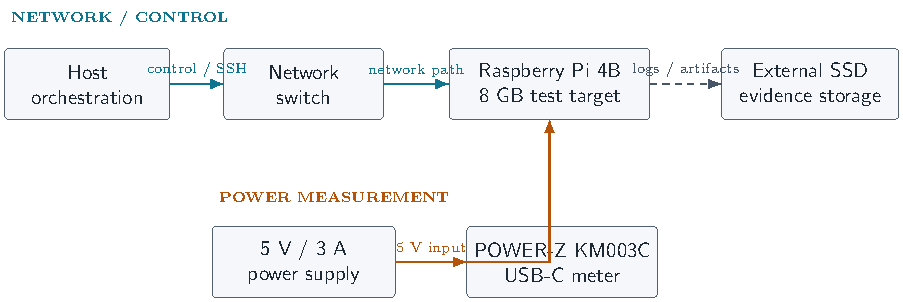
\includegraphics[width=.78\textwidth]{figures/experiment_setup_schematic.pdf}
\caption{Supply, inline POWER-Z KM003C and Raspberry Pi 4B, with Ethernet orchestration through a switch and external evidence storage. Roles are schematic; power is whole-device load-side USB input, not CPU-only power.}
\label{fig:experimentdesign}\end{figure*}
